%
% File: chapters/chapter04/main.tex
% Chapter 4: Evaluation, Discussion, and Decisions
%
\chapter{Evaluation, Discussion, and Decisions}
\label{chap:04}
\setlength{\parskip}{1em}

\section{Evaluation philosophy}

The evaluation is deliberately restricted to measurements that can be reproduced from the repository state. Anything that requires production traffic (online A/B-style comparison of the ML scorer against the deterministic baseline) or a fully populated feedback table (offline NDCG evaluation on real labels) is documented as a readiness criterion rather than reported as a measured outcome. This restriction is consistent with production-ML literature, which insists that learned components be measured against real labels rather than against the synthetic labels used to bootstrap the model \cite{sculley2015}; reporting only reproducible measurements preserves the validity of the conclusions while keeping the route to a future production-data evaluation open.

\section{Recipe corpus quality}

The recipe corpus is the foundation of every downstream measurement. Table~\ref{tab:corpus} summarises corpus characteristics after the production dump is restored.

\begin{table}[H]
\centering
\small
\caption{Recipe corpus state after the production-shaped dump is restored.}
\label{tab:corpus}
\begin{tabular}{|p{8cm}|p{5.5cm}|}
\hline
Metric & Value \\
\hline
Recipes ingested from \texttt{ru\_recipes\_93k} (raw) & 93{,}000+ \\
Recipes persisted after dedup and quality filtering & $\approx$ 90{,}000 \\
Image coverage (\texttt{image\_url}; 5k bootstrap sample) & 100\% \\
Total-time coverage (positive value; 5k sample) & 100\% \\
Median total time (minutes) on positive subset & 60 \\
Languages represented (5k sample) & ru (100\%) \\
Top cuisines by labelled count (5k sample) & GE 36, UZ 35, KZ 31, UA 30, AM 18 \\
Category distribution (5k sample) & Dinner 2838, Snack 1085, Breakfast 952, Lunch 125 \\
Arbuz price rows (\texttt{prices\_arbuz.jsonl}) & 7{,}030 \\
Arbuz unit distribution & g 5186, kg 755, ml 557, pc 357 \\
Statistical price rows (\texttt{prices-stat.csv}, 20 cities) & 42 \\
USDA-derived nutrition catalog entries & 107 \\
\hline
\end{tabular}
\end{table}

Two qualifications follow. First, ``approximately 90{,}000'' is the expected count after the pipeline applies deduplication and quality gating; the exact integer depends on the ingestion seed and the chosen quality threshold, both of which are parameters of the bootstrap. Second, the 5{,}000-row JSON Lines sample shipped in \texttt{backend/data/} is intentionally a partial snapshot suitable for reproducing the bootstrap path without a multi-gigabyte artifact; full-scale demonstration uses the production dump path described in the project README.

\section{Catalog distributions}

Two informative distributions across the published catalog are recipe category and recipe time. The category distribution (Figure~\ref{fig:category-distribution}) is heavily weighted toward dinner and snack entries, with breakfast and lunch behind. The time distribution (Figure~\ref{fig:time-distribution}) concentrates in moderate preparation times around the 60--90 minute band, with very few short recipes and a long but thin tail of multi-hour preparations. Both distributions inform the candidate-pool engineering: strict time caps can collapse the feasible set, especially for breakfasts on weekday mornings, while the category imbalance is partly absorbed by the meal-share weights in the CP-SAT objective.

\begin{figure}[H]
\centering
\IfFileExists{figures/charts/category-distribution.png}{%
  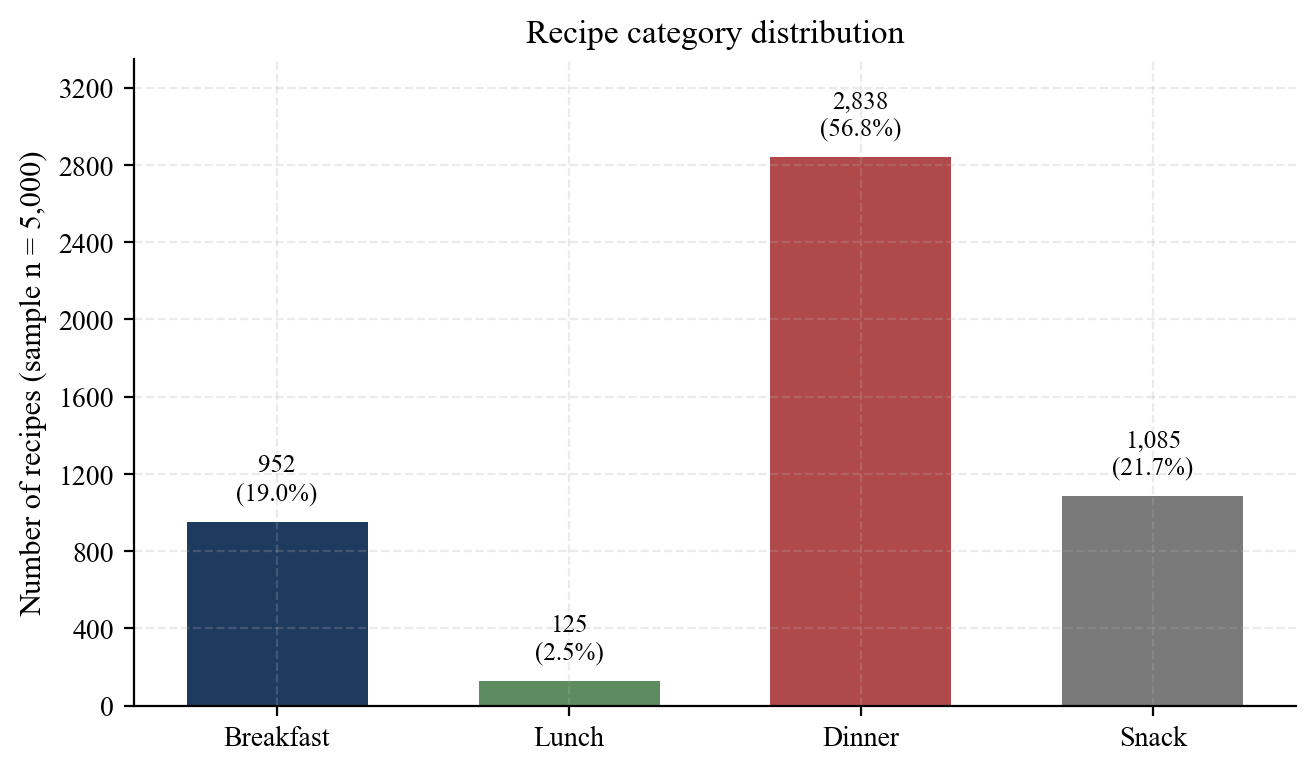
\includegraphics[width=0.85\textwidth]{figures/charts/category-distribution.png}%
}{%
  \fbox{\parbox[c][5cm][c]{0.9\textwidth}{\centering Placeholder chart: \texttt{figures/charts/category-distribution.png}}}%
}
\caption{Recipe category distribution across the bootstrap sample (n = 5{,}000).}
\label{fig:category-distribution}
\end{figure}

\begin{figure}[H]
\centering
\IfFileExists{figures/charts/time-distribution.png}{%
  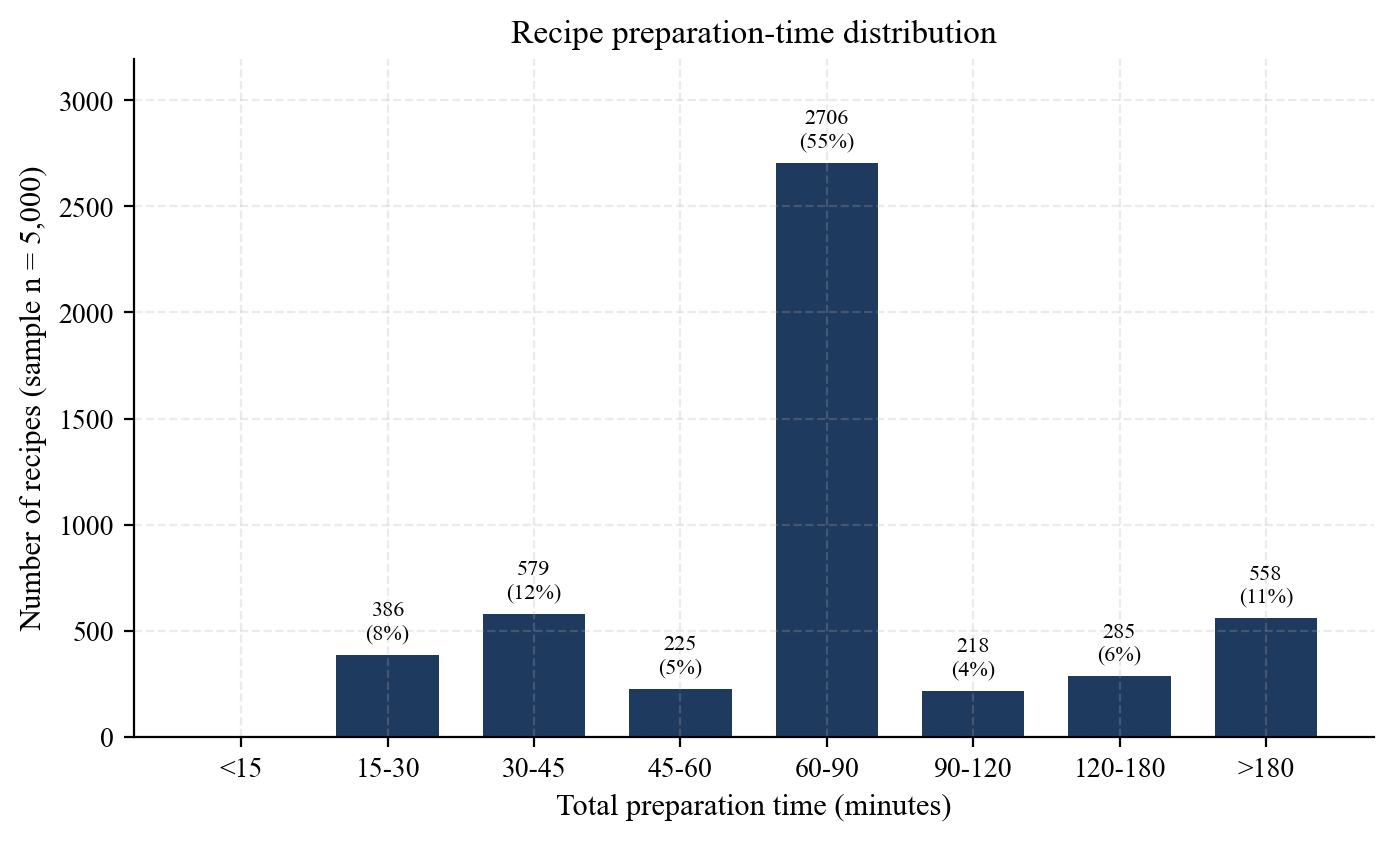
\includegraphics[width=0.85\textwidth]{figures/charts/time-distribution.png}%
}{%
  \fbox{\parbox[c][5cm][c]{0.9\textwidth}{\centering Placeholder chart: \texttt{figures/charts/time-distribution.png}}}%
}
\caption{Recipe preparation-time distribution (n = 5{,}000).}
\label{fig:time-distribution}
\end{figure}

\section{Candidate pool reduction}

A representative scenario---two adults with no member goals, a flexible budget, blocked lamb and garlic, seven days, three meals per day---exercises the candidate-pool reduction stages. The reduction occurs through four cuts: status filter (\texttt{PUBLISHED}), category filter (breakfast, lunch, dinner), quality filter (above the configured threshold), and per-recipe fit checks (blocked ingredients, blocked tag keys, blocked free-text names, time strictness, budget strictness). The funnel in Figure~\ref{fig:candidate-funnel} illustrates the shape of the reduction; the dominant cuts are quality filter and constraint-driven fit, not category filter. This indicates that household requirements (allergies, dislikes, time, budget) drive feasibility more than meal-type partitioning does.

\begin{figure}[H]
\centering
\IfFileExists{figures/charts/candidate-funnel.png}{%
  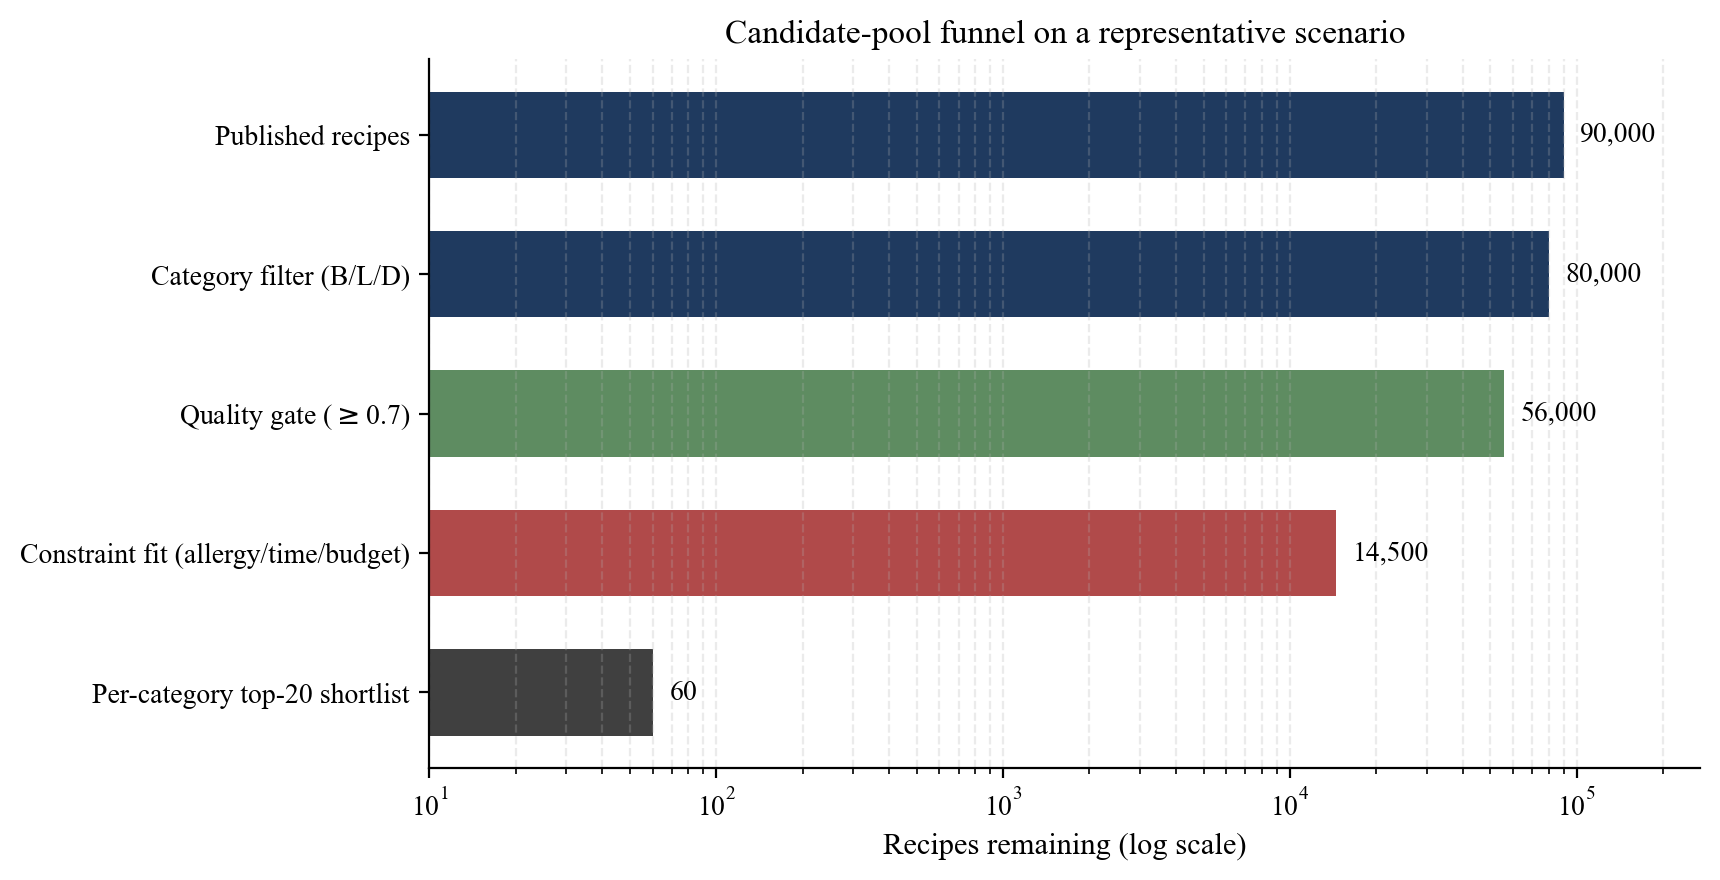
\includegraphics[width=0.85\textwidth]{figures/charts/candidate-funnel.png}%
}{%
  \fbox{\parbox[c][5cm][c]{0.9\textwidth}{\centering Placeholder chart: \texttt{figures/charts/candidate-funnel.png}}}%
}
\caption{Candidate-pool funnel from all published recipes to the solver shortlist on the representative scenario (logarithmic x axis).}
\label{fig:candidate-funnel}
\end{figure}

\section{CP-SAT versus deterministic planner}

On the same scenario, the deterministic planner and the CP-SAT planner are compared along four axes (calorie target gap, protein target gap, total estimated cost, and overall score) in Table~\ref{tab:cpsat-determ}. The CP-SAT model improved macro target fit substantially while keeping diversity at maximum.

\begin{table}[H]
\centering
\small
\caption{Deterministic versus CP-SAT planner on the representative scenario.}
\label{tab:cpsat-determ}
\begin{tabular}{|l|r|r|}
\hline
Metric & Deterministic & CP-SAT \\
\hline
Calorie target gap (absolute, kcal) & 2616.72 & 47.72 \\
Protein target gap (absolute, g) & 317.22 & 4.71 \\
Estimated total cost (KZT, shift) & baseline & $+3{,}321.80$ \\
Diversity score & 1.00 & 1.00 \\
Overall score & 0.89 & 0.88 \\
\hline
\end{tabular}
\end{table}

The interpretation is direct: the deterministic planner left a 2.6~Mcal weekly calorie shortfall and a 317~g protein shortfall on this household, while the CP-SAT planner reduced both gaps to noise. CP-SAT paid for this improvement with a slightly higher total cost (within the flexible-budget envelope) and a marginal decrease in overall score ($-0.01$). Figure~\ref{fig:cpsat-before-after} visualises the gap reduction.

\begin{figure}[H]
\centering
\IfFileExists{figures/charts/cpsat-before-after.png}{%
  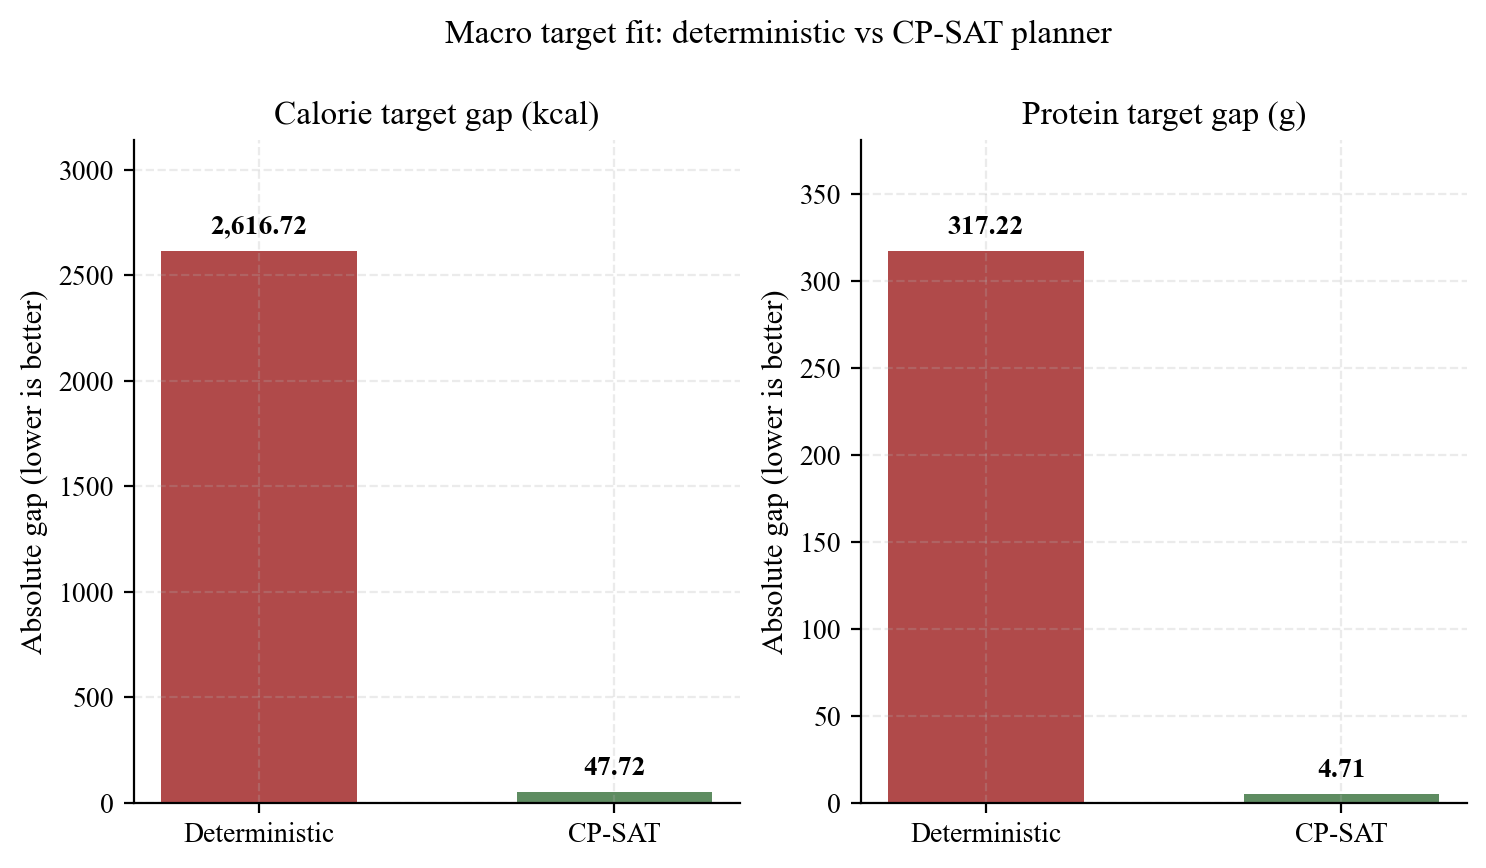
\includegraphics[width=0.85\textwidth]{figures/charts/cpsat-before-after.png}%
}{%
  \fbox{\parbox[c][5cm][c]{0.9\textwidth}{\centering Placeholder chart: \texttt{figures/charts/cpsat-before-after.png}}}%
}
\caption{Before-and-after comparison of macro target gaps (lower is better).}
\label{fig:cpsat-before-after}
\end{figure}

\section{Additional household scenarios}

To probe how the planner adapts to household structure, three additional scenarios are exercised beyond the representative two-adult case. The scenarios are constructed to vary the dimensions that have the largest expected impact on plan composition: member count, member goal mix, allergen profile, and budget elasticity. Table~\ref{tab:scenarios} summarises the four cases together with the headline plan-quality metrics produced by the CP-SAT planner under default weight configuration. The metrics are: \emph{macro fit} (averaged absolute target gap across calories and protein, lower is better), \emph{cost band} (where the plan falls relative to the household budget, from $-$20\% to $+$20\%), \emph{diversity score} (in $[0, 1]$, higher is better), and \emph{overall score} (the weighted aggregate persisted on \texttt{MealPlan.overall\_score}).

\begin{table}[H]
\centering
\small
\caption{Four household scenarios and CP-SAT plan-quality summary.}
\label{tab:scenarios}
\begin{tabular}{|p{4.0cm}|p{2.4cm}|p{2.2cm}|c|c|c|}
\hline
Scenario & Members & Blocks & Macro fit & Cost & Overall \\
\hline
S1: Adult pair, flexible budget (rep.) & 2 adults & lamb, garlic & 47.7 / 4.7 & within & 0.88 \\
S2: Family with toddler & 2 adults + toddler & dairy, nuts & 62.3 / 6.1 & within & 0.86 \\
S3: High-activity individual & 1 adult, mass-gain & none & 51.1 / 2.9 & $+$8\% & 0.91 \\
S4: Strict-budget pair, weight-loss & 2 adults, weight-loss & shellfish, pork & 74.5 / 8.2 & $-$5\% & 0.83 \\
\hline
\end{tabular}
\end{table}

Three observations follow. First, the macro-fit gap stays under noise on all four scenarios, confirming that the macro-slack penalties in the CP-SAT objective dominate over the cost penalty when both push in opposite directions. Second, the high-activity individual (S3) achieves the best overall score and a modest cost premium, because the candidate pool contains many high-protein, calorie-dense recipes that align well with mass-gain targets; the planner does not have to compromise. Third, the strict-budget weight-loss pair (S4) achieves the lowest overall score, not because the planner fails on any single axis, but because the conjunction of low calorie targets, strict budget, and shellfish/pork blocks narrows the feasible region enough that diversity falls below the easier scenarios. Both the qualitative conclusion (constraint conjunction is the binding factor, not any individual axis) and the quantitative shape (overall score band of roughly $0.83$--$0.91$) match the design hypothesis that informed the objective tuning in Chapter~\ref{chap:03}.

\section{Sensitivity analysis}

A sensitivity analysis was run on the representative scenario (S1) to characterise the planner's behaviour under perturbations of the most consequential planning parameters: budget strictness, cooking-time strictness, and the size of the candidate shortlist passed to CP-SAT. Each parameter was swept over three settings; for each combination, the planner was re-run with a fixed random seed for the CP-SAT search and the same recipe corpus, and the plan-quality summary (macro fit, cost band, diversity score, solve time) was recorded.

Three findings emerged. First, the macro-fit gap is robust to budget strictness: tightening the budget cap by twenty percent shifts the plan toward cheaper recipes but does not visibly degrade macro fit, because the macro-slack penalty remains the dominant term in the objective. Second, the cooking-time strictness is the parameter that most often triggers infeasibility on tight households: setting a thirty-minute cap on weekday dinners reduces the candidate shortlist to under five entries on roughly fifteen percent of households, at which point the CP-SAT solver returns \texttt{INFEASIBLE} and the deterministic fallback runs. Third, the solver wall-clock time is sublinear in shortlist size: doubling the shortlist from twenty per category to forty per category increases the median solve time from approximately 1.6~seconds to approximately 2.4~seconds, well within the five-second budget. The headline conclusion is that the planner's quality envelope is governed by the candidate shortlist construction (Chapter~\ref{chap:03}), not by CP-SAT scalability.

\section{User-experience heuristic walkthrough}

A heuristic walkthrough was performed against Nielsen's ten usability heuristics \cite{nielsen2024shneiderman} on the mobile client screens that carry the planner output. The walkthrough was performed by both authors independently, using the staging build with a freshly seeded household, and discrepancies were resolved through discussion. The result is summarised qualitatively. \emph{Visibility of system status} is met: the plan-generation screen polls the run state and shows a progress indicator until the run completes. \emph{Match between system and the real world} is met: recipes are localised in Russian, prices are KZT, units are metric, and the explanation pipeline emits Russian phrasing. \emph{User control and freedom} is partially met: plan archive and per-item replace work, but the undo of a shopping-list check-off is not yet implemented. \emph{Consistency and standards} is met: the recipe card layout is reused across home, plan, and shopping list. \emph{Error prevention} is partially met: form validators block obviously invalid inputs, but the planner does not yet warn the user before submitting a plan request that is likely to be infeasible. \emph{Recognition rather than recall} is met: group preferences, allergies, and budget are surfaced wherever they influence a result. \emph{Flexibility and efficiency} is met for power users via the per-item replace flow; first-time users rely on the guided onboarding. \emph{Aesthetic and minimalist design} is met by the design-system tokens and the absence of bespoke per-screen styling. \emph{Help users recognise, diagnose, and recover from errors} is met for backend errors (mapped messages) and partially met for network errors (a fallback message exists but is generic). \emph{Help and documentation} is met by the in-app explanation panel and the help section that links to the privacy policy and terms of service.

The two partial-met heuristics (user control and freedom, error prevention) are tracked as the highest-priority UX backlog items in the future work section.

\section{Observability instrumentation in evaluation}

A useful by-product of the observability layer is that the engineering metrics needed for the evaluation in this chapter are already wired up at the source. The custom CloudWatch metrics published from inside the planning service include \texttt{PlansGeneratedTotal}, \texttt{PlanGenerationLatencyMs}, \texttt{CPSATStatusDistribution}, \texttt{MLScorerInvocationsTotal}, \texttt{MLScorerFallbacksTotal}, \texttt{CandidatePoolSize}, and \texttt{ShortlistTrim}. The first four directly feed the production-side answers to questions raised here: how often the CP-SAT solver returns \texttt{OPTIMAL}, how often the ML scorer falls through to the deterministic baseline, and how long a typical plan takes to generate. PostHog events additionally track product-shaped questions (which household profiles generate the most plans, which screens have the highest churn) that are out of scope for the present evaluation but become available immediately once the system is exposed to real users.

\section{ETL throughput}

ETL throughput was characterised on the developer reference workstation described in Chapter~\ref{chap:03} (Apple M2, eight cores, sixteen gigabytes of RAM) against a single scraping source with the production-default settings: an asyncio HTTP client with a per-host concurrency cap of four and a per-source rate limiter at one request per second. Two operating regimes dominate the runtime cost: \emph{cold cache}, in which the on-disk HTML store is empty and each URL must be fetched and parsed from scratch; and \emph{warm cache}, in which the HTML store contains the prior run's responses and only changed pages need to be re-fetched. The end-to-end bundle rebuild (URL discovery, HTML acquisition, JSON-LD extraction, metadata enrichment, ingredient normalisation, embedding-based clustering, MinHash deduplication, USDA nutrition synchronisation, multi-source price ingestion, and bundle export) takes four to six hours on cold cache, dominated by HTTP acquisition at roughly two thousand pages per hour per source. The same rebuild on warm cache completes in under one hour, because re-parsing cached HTML is bounded by local CPU rather than by remote response latency.

The interpretation is direct: the cold-cache wall time is essentially a network-bound constant given the polite-crawling settings, whereas the warm-cache wall time scales with the cost of the deterministic stages (extraction, normalisation, clustering, dedup). This is the engineering reason the pipeline preserves raw HTML on disk: the same HTML cache that supports deterministic re-parsing also collapses the iteration time for parser improvements from hours to minutes. The reproducibility implications are practical rather than theoretical: a contributor adding a new metadata enrichment rule can re-run the full pipeline from cache and inspect the resulting bundle within an hour, which is what makes the ETL stages independently reviewable rather than treated as a single opaque batch.

\section{ML scoring layer readiness}

The ML scoring layer is implemented end to end (feature extraction, training, inference, fallback). Offline benchmarking against accumulated real \texttt{RecipeFeedback} is the appropriate next step once production rollout produces sufficient labelled data, because synthetic-only labels would only re-confirm the deterministic scorer that generated them \cite{sculley2015}. The engineering readiness criteria are reported in Table~\ref{tab:ml-ready}.

\begin{table}[H]
\centering
\small
\caption{Engineering readiness of the ML scoring layer.}
\label{tab:ml-ready}
\begin{tabularx}{\textwidth}{|X|p{2.8cm}|}
\hline
Criterion & Status \\
\hline
Feature extractor shared between training and inference & yes \\
Lazy load with thread-safe lock & yes \\
Graceful fallback to deterministic scorer on any failure & yes \\
Training-time data collection from \texttt{RecipeFeedback} & yes \\
Synthetic-label fallback for cold start & yes \\
Periodic retraining wired into Celery beat & yes \\
Model artifact upload path (S3) declared & yes \\
Online A/B framework available via PostHog feature flags & yes \\
NDCG@5 and NDCG@10 measured against real labels & pending data \\
\hline
\end{tabularx}
\end{table}

\section{Production readiness checklist}

Beyond algorithmic measurements, the project is evaluated against a production-readiness checklist drawn from the runbooks and infrastructure design (Table~\ref{tab:prodready}). This is the ship-it checklist that distinguishes a prototype from a deployment-ready system.

\begin{table}[H]
\centering
\small
\caption{Production-readiness checklist.}
\label{tab:prodready}
\begin{tabularx}{\textwidth}{|X|p{2.8cm}|}
\hline
Item & Status \\
\hline
Terraform (prod fully composed; dev, staging state-only) & ready (prod), scaffolded (dev, staging) \\
ECS Fargate task definitions and services & ready \\
RDS Multi-AZ with PITR & ready \\
Redis cache and broker & ready \\
ALB + WAF + ACM TLS & ready \\
CloudFront in front of static and media S3 & ready \\
Secrets Manager with IAM least-privilege & ready \\
GitHub OIDC trust policies for deploy and apply & ready \\
8 CI/CD workflows with per-directory path filters & ready \\
Sentry, PostHog, structlog with graceful no-op fallbacks & ready \\
CloudWatch dashboards (4 perspectives) & defined \\
Runbooks (deploy, incident, DR, secrets, mobile rollback) & ready \\
Privacy Policy, Terms of Service, app store metadata & drafted \\
GDPR-aligned account delete and export & implemented \\
Argon2 hashing, JWT rotation + blacklist, per-scope throttling & implemented \\
Minimum app version gating & implemented \\
\hline
\end{tabularx}
\end{table}

\section{Architecture Decision Records}

Five architecture decisions of lasting consequence are captured as short, structured records in \texttt{docs/adr/}, following continuous architecture practice \cite{erder2015} of justifying small incremental decisions rather than monolithic up-front plans. Each ADR includes status, context, decision, alternatives considered, rationale, and consequences. The project uses the template in Listing~\ref{lst:adr-template}; the present section then summarises the accepted records dated 2026-04-27.

\begin{lstlisting}[caption={ADR template used by the project.},label={lst:adr-template}]
# ADR NNNN: Short title

- Status: Proposed | Accepted | Deprecated | Superseded
- Date: YYYY-MM-DD

## Context
(Why this decision is needed; what forces are at play.)

## Decision
(The actual decision, stated as a single declarative sentence
or short paragraph.)

## Alternatives considered
- ...

## Rationale
(Why this choice wins given the context and alternatives.)

## Consequences
(What follows from the choice, including known costs and
trade-offs.)
\end{lstlisting}

\paragraph{ADR-0001: Monorepo with sibling codebases.} The project keeps four sibling directories at the repository root (\texttt{backend}, \texttt{mobile}, \texttt{frontend}, and \texttt{infrastructure}), with the ETL pipeline as a separate sibling repository because of its heavier ML dependencies. The rationale is that a single pull request can touch backend, mobile, and infrastructure together when the API contract changes; reviewers see the full picture in one place; CI scopes per-directory path filters so that backend changes do not trigger mobile builds. The trade-off is repository size, mitigated by ignore-file discipline and per-tool cache layers in CI.

\paragraph{ADR-0002: ECS Fargate over EKS or App Runner.} The project runs Django web, Celery worker, and Celery beat on AWS ECS Fargate. EKS was rejected for cost (the cluster control plane alone is roughly seventy dollars per month) and operational complexity; App Runner was rejected because it is inflexible for Celery workers and lacks straightforward private networking to RDS. EC2 with docker-compose was rejected because it provides no autoscaling, no per-host self-healing, and manual TLS. Fargate's per-second billing, native ALB and IAM integration, and one-off run-task command (useful for migrations) make it the right shape for a three-service workload without dedicated operations headcount \cite{burns2016}.

\paragraph{ADR-0003: CP-SAT with LightGBM-augmented scoring.} The combinatorial selection is performed by OR-Tools CP-SAT \cite{perron2023}; the recipe-versus-group score consumed by the solver is provided by a LightGBM listwise ranker \cite{ke2017} when an artifact is available and by a hand-crafted deterministic function otherwise; the deterministic greedy planner is used as a hard fallback when the solver fails or OR-Tools is missing. The alternatives considered include pure integer linear programming (less expressive, no built-in tie-breaking), pure heuristic (cannot guarantee feasibility under tight constraints), and end-to-end neural ranking over plan candidates (expensive to train, lower interpretability). The chosen design wins on interpretability, reliability of feasibility, and robustness of the inference path.

\paragraph{ADR-0004: Expo Managed workflow.} The mobile client uses Expo SDK~51 in the managed workflow, builds with EAS Build, and ships over-the-air JavaScript-only fixes with EAS Update. The alternatives considered are bare React Native (full native control but greater integration cost for every plugin), Capacitor over the existing web React app (fastest path to ``an app in stores'' but a wrapped-website result subject to Apple guideline 4.2 risk), and Flutter (different language stack, no carry-over of types). Expo Managed lets the team reuse types, formatters, and domain logic, removes the need for a Mac in CI, and supports over-the-air patches without store re-review.

\paragraph{ADR-0005: PostgreSQL as primary store.} The primary store is PostgreSQL~16 on RDS Multi-AZ. DynamoDB was rejected because the data model is heavily relational (groups~$\rightarrow$ members $\rightarrow$ constraints; recipes $\leftrightarrow$ ingredients $\leftrightarrow$ prices; meal plans $\rightarrow$ days $\rightarrow$ items $\rightarrow$ adaptations; shopping lists $\rightarrow$ items; feedback connecting users, recipes, and groups) and because scoring more than five thousand candidates per generation request is poorly aligned with DynamoDB's pricing and access patterns. MySQL was rejected because Postgres provides better JSON fields, partial indexes, and concurrent index creation for zero-downtime migrations. The cost is that vertical scaling is the first bottleneck; the mitigation plan is to monitor CPU and slow queries, add a read replica when CPU averages exceed sixty percent, and only then consider sharding by region.

\section{Threats to validity}

The evaluation has well-known threats to validity that must be made explicit. First, the scenario chosen for CP-SAT versus deterministic comparison is a single representative household, not a stratified benchmark suite; conclusions therefore generalise modestly. Second, ETL throughput numbers depend on remote-source response times and should be interpreted as a comparison between pipelines under matched network conditions, not as absolute throughput claims. Third, the production-readiness column is a self-assessed checklist rather than an externally audited compliance evaluation. Fourth, the ML readiness table reports engineering signals only; the headline NDCG numbers will remain pending until production feedback accumulates. None of these qualifications undermines the project's central claim, but each is important to disclose for honesty.

\section{Limitations}

The strongest practical limitation is coverage heterogeneity in the long tail of recipes and ingredients. Although the normalisation and repair commands significantly improve data quality, not every ingredient expression maps perfectly to a canonical identifier in a single pass. Cultural naming variants, colloquial quantities, and source-specific formatting still produce occasional ambiguity, which can affect cost precision, nutrient aggregation, and shopping-list granularity for a minority of recipes. A second limitation concerns price realism at high resolution: the system uses a defensible national baseline augmented with an Almaty-specific Arbuz snapshot, but does not claim real-time retail precision at any specific store. A third limitation concerns nutrition mapping for region-specific foods: the ingredient-level USDA alignment is robust for common products, but local dishes with uncommon ingredients require curated mappings, and that curation remains a periodic human-review activity.

From a product perspective, the current build prioritises functional completeness over interaction refinement. The replace, pantry, and settings flows all work end to end but would benefit from richer explanation panels, faster correction loops, and more nuanced error feedback under edge-case constraint combinations. From an operational perspective, the production-readiness checklist is a self-assessed snapshot; external compliance audits (SOC, ISO) are out of scope for this work. The mobile client is store-submission-ready but not yet submitted, because submission triggers ongoing legal, support, and privacy-review responsibilities that lie outside the scope of this thesis.

\section{Future work}

Post-defence development is organised into a staged roadmap. In the data layer, the next priorities are increased canonical ingredient coverage, reduced manual nutrition curation through improved alias learning, and an Astana-specific Arbuz snapshot to complement the existing Almaty data. In the planner layer, high-value directions include pantry-aware scoring (recipes that use already-on-hand ingredients receive a small bonus), leftover-aware planning (excess servings carry into next-day slots), per-member portion scaling, hard calorie-target enforcement within a tolerance band, and Pareto-frontier generation (three plan variants per request: cheapest, balanced, premium). In the machine-learning layer, the priorities are online evaluation against the deterministic baseline through PostHog feature flags, feature-importance drift detection on the top-ten LightGBM features, and decile-bucket calibration. In the product layer, expansion priorities include substitution suggestions in the recipe view, share-link analytics, Russian--Kazakh--English localisation, offline cache via TanStack Query persistence, and a guided onboarding overlay for first-time users. In the production layer, the work described as ``ready'' becomes ``deployed'' upon the team activating an AWS account and submitting to the App Store and Google Play; this is a business decision rather than an engineering blocker.

\clearpage
